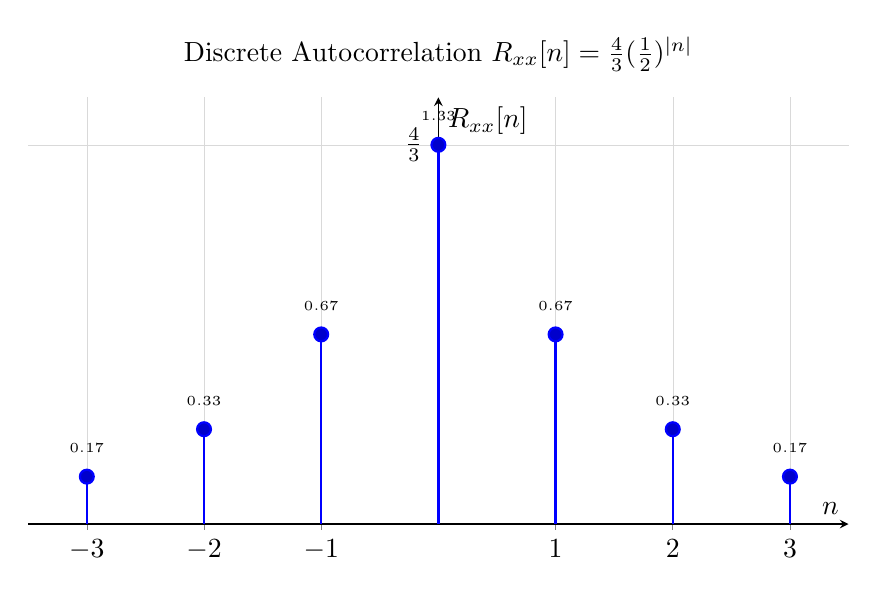
\begin{tikzpicture}
	\pgfplotsset{impulse/.style={ycomb,blue,thick,mark=*,mark size=2.5pt}}
	\begin{axis}[
		width=12cm,
		height=7cm,
		title={Discrete Autocorrelation $R_{xx}[n] = \frac{4}{3}(\frac{1}{2})^{|n|}$},
		xlabel={$n$},
		ylabel={$R_{xx}[n]$},
		axis lines=middle,
		xmin=-3.5, xmax=3.5,
		ymin=0, ymax=1.5,
		xtick={-3,-2,-1,0,1,2,3},
		ytick={1.333},
		yticklabels={$\frac{4}{3}$},
		grid=major,
		grid style={line width=.1pt, draw=gray!30},
		]
		\addplot+[impulse, samples at={-3,...,3}, nodes near coords,
		every node near coord/.style={font=\tiny, text=black,
			yshift=5pt, anchor=south},] {(4/3)*(1/2)^abs(x)};
	\end{axis}
\end{tikzpicture}